\begin{frame}
\frametitle{Effect of the Experimental Covariance}

\begin{columns}[T]

%%%%%%%%%%%%%%%%%%%%%%%%%%%%%%%%%%%%

\column{0.42\textwidth}

\small

Our study focuses on the experimental systematic covariance,

\vspace{-0.1cm}

\[
\boxed{\Sigma_{\rm sys}}
\]

\vspace{-0.1cm}

which determines how systematic uncertainties are correlated among experimental data points.

\vspace{0.1cm}

Different covariance models are investigated:

\begin{itemize}
\item Diagonal
\item Compound Symmetry
\item Radial Basis Function (RBF)
\end{itemize}

%%%%%%%%%%%%%%%%%%%%%%%%%%%%%%%%%%%%

\column{0.58\textwidth}

\centering

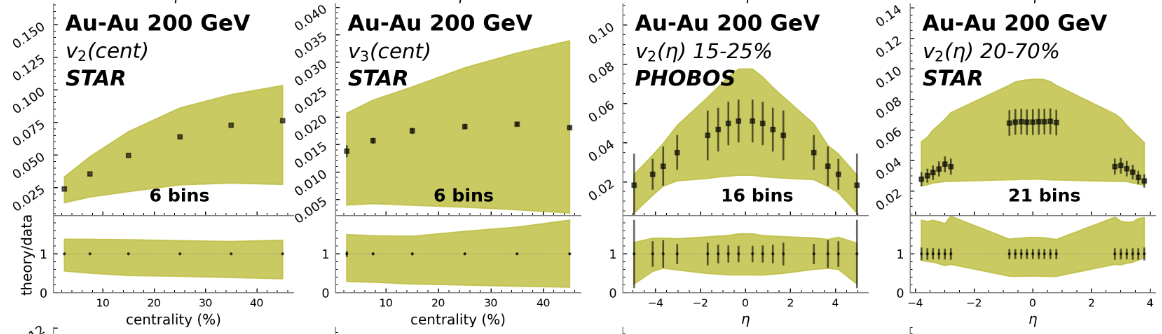
\includegraphics[width=.95\linewidth]{img/Au-Au-prior.png}

\vspace{0.15cm}

{\Large $\Downarrow$}

\small Bayesian calibration

\vspace{0.15cm}

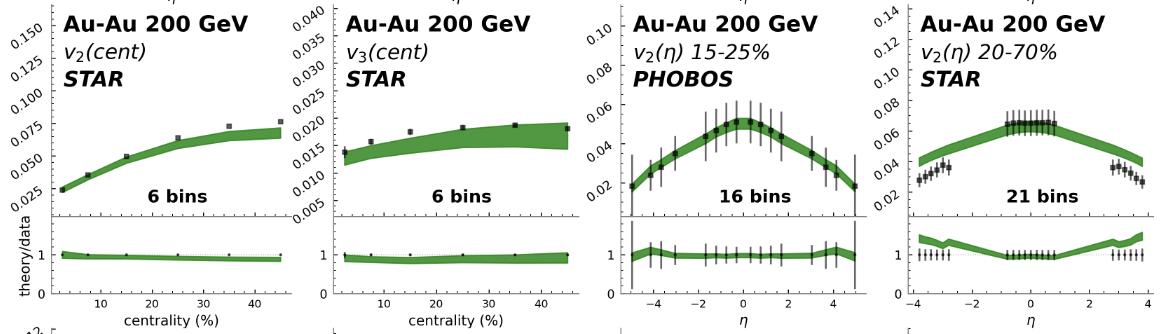
\includegraphics[width=.95\linewidth]{img/Au-Au-posterior.png}

\end{columns}

\vspace{0.4cm}
\small
Changing $\Sigma_{\rm sys}$ modifies the likelihood and therefore the posterior constraints.

\end{frame}